\chapter{Graphics}
\label{graphics}

\index{AWT}
\index{java.awt}

The Java library includes a simple package for drawing 2D graphics, called \java{java.awt}.
{\bf AWT} stands for ``Abstract Window Toolkit''.
We are only going to scratch the surface of graphics programming.
You can read more about it in the Java tutorials at \url{https://thinkjava.org/java2d}.


\section{Creating Graphics}

\index{Canvas}
\index{class!Canvas}
\index{Graphics}
\index{class!Graphics}

There are several ways to create graphics in Java; the simplest way is to use \java{java.awt.Canvas} and \java{java.awt.Graphics}.
A \java{Canvas} is a blank rectangular area of the screen onto which the application can draw.
The \java{Graphics} class provides basic drawing methods such as \java{drawLine}, \java{drawRect}, and \java{drawString}.

Here is an example program that draws a circle using the \java{fillOval} method:

\begin{code}
import java.awt.Canvas;
import java.awt.Graphics;
import javax.swing.JFrame;

public class Drawing extends Canvas {
\end{code}

\begin{code}
    public static void main(String[] args) {
        JFrame frame = new JFrame("My Drawing");
        Drawing drawing = new Drawing();
        drawing.setSize(400, 400);
        frame.add(drawing);
        frame.pack();
        frame.setVisible(true);
    }

    public void paint(Graphics g) {
        g.fillOval(100, 100, 200, 200);
    }
}
\end{code}

The \java{Drawing} class extends \java{Canvas}, so it has all the methods provided by \java{Canvas}, including \java{setSize}.
You can read about the other methods in the documentation, which you can find by doing a web search for ``Java Canvas''.

\index{JFrame}
\index{class!JFrame}

In the \java{main} method, we:

\begin{enumerate}

\item Create a \java{JFrame} object, which is the window that will contain the canvas.

\item Create a \java{Drawing} object (which is the canvas), set its width and height, and add it to the frame.

\item Pack the frame (resize it) to fit the canvas, and display it on the screen.
\end{enumerate}

\index{paint}

Once the frame is visible, the \java{paint} method is called whenever the canvas needs to be drawn; for example, when the window is moved or resized.
The application doesn't end after the \java{main} method returns; instead, it waits for the \java{JFrame} to close.
If you run this code, you should see a black circle on a gray background.


\section{Graphics Methods}

\index{coordinate}

You are probably used to Cartesian {\bf coordinates}, where $x$ and $y$ values can be positive or negative.
In contrast, Java uses a coordinate system where the origin is in the upper-left corner.
That way, $x$ and $y$ can always be positive integers.
Figure~\ref{fig.coordinates} shows these coordinate systems side-by-side.

\begin{figure}[!ht]
\begin{center}
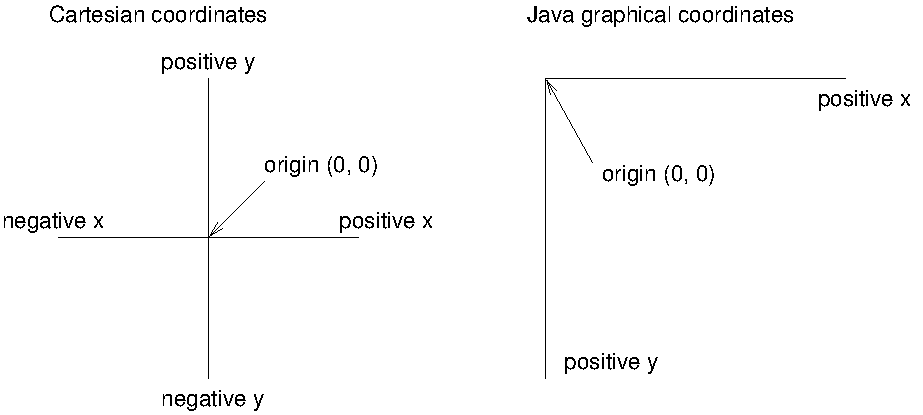
\includegraphics[width=5in]{figs/coordinates.pdf}
\caption{Diagram of the difference between Cartesian coordinates and Java graphical coordinates.}
\label{fig.coordinates}
\end{center}
\end{figure}

\index{pixel}

Graphical coordinates are measured in {\bf pixels}; each pixel corresponds to a dot on the screen.

To draw on the canvas, you invoke methods on a \java{Graphics} object.
You don't have to create the \java{Graphics} object; it gets created when you create the \java{Canvas}, and it gets passed as an argument to \java{paint}.

The previous example used \java{fillOval}, which has the following signature:

\begin{code}
/**
 * Fills an oval bounded by the specified rectangle with
 * the current color.
 */
public void fillOval(int x, int y, int width, int height)
\end{code}

\index{bounding box}

The four parameters specify a {\bf bounding box}, which is the rectangle in which the oval is drawn.
\java{x} and \java{y} specify the location of the upper-left corner of the bounding box.
The bounding box itself is not drawn (see Figure~\ref{fig.circle}).

\begin{figure}[!ht]
\begin{center}
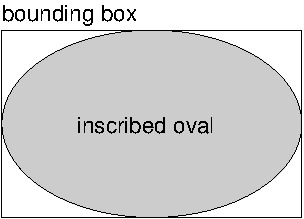
\includegraphics{figs/circle.pdf}
\caption{Diagram of an oval inside its bounding box.}
\label{fig.circle}
\end{center}
\end{figure}

\index{Color}

To choose the color of a shape, invoke \java{setColor} on the \java{Graphics} object:

\begin{code}
g.setColor(Color.RED);
\end{code}

The \java{setColor} method determines the color of everything that gets drawn afterward.
\java{Color.red} is a constant provided by the \java{Color} class; to use it you have to \java{import java.awt.Color}.
Other colors include:

\begin{stdout}
BLACK       BLUE      CYAN     DARKGRAY   GRAY    LIGHTGRAY
GREEN       MAGENTA   ORANGE   PINK       WHITE   YELLOW
\end{stdout}

\index{RGB}

You can create your own colors by specifying the red, green, and blue ({\bf RGB}) components.
For example:

\begin{code}
Color purple = new Color(128, 0, 128);
\end{code}

Each value is an integer in the range 0 (darkest) to 255 (lightest).
The color \java{(0, 0, 0)} is black, and \java{(255, 255, 255)} is white.

You can set the background color of the \java{Canvas} by invoking \java{setBackground}:

\begin{code}
canvas.setBackground(Color.white);
\end{code}


\section{Example Drawing}

\index{Mickey Mouse}

Suppose we want to draw a ``Hidden Mickey'', which is an icon that represents Mickey Mouse (see \url{https://en.wikipedia.org/wiki/Hidden_Mickey}).
We can use the oval we just drew as the face, and then add two ears.
To make the code more readable, let's use \java{Rectangle} objects to represent bounding boxes.

Here's a method that takes a \java{Rectangle} and invokes \java{fillOval}:

\begin{code}
public void boxOval(Graphics g, Rectangle bb) {
    g.fillOval(bb.x, bb.y, bb.width, bb.height);
}
\end{code}

And here's a method that draws Mickey Mouse:

\begin{code}
public void mickey(Graphics g, Rectangle bb) {
    boxOval(g, bb);

    int dx = bb.width / 2;
    int dy = bb.height / 2;
    Rectangle half = new Rectangle(bb.x, bb.y, dx, dy);

    half.translate(-dx / 2, -dy / 2);
    boxOval(g, half);

    half.translate(dx * 2, 0);
    boxOval(g, half);
}
\end{code}

The first line draws the face.
The next three lines create a smaller rectangle for the ears.
We \java{translate} the rectangle up and left for the first ear, then to the right for the second ear.
The result is shown in Figure~\ref{fig.mickey}.

\begin{figure}[!ht]
\begin{center}

\includegraphics[height=2in]{figs/mickey.png}
\caption{A ``Hidden Mickey'' drawn using Java graphics.}
\label{fig.mickey}
\end{center}
\end{figure}

You can read more about \java{Rectangle} and \java{translate} in Chapter~\ref{mutable}.
See the exercises at the end of this appendix for more example drawings.


\section{Vocabulary}

\begin{description}

\term{AWT}
The ``Abstract Window Toolkit'', a Java package for creating graphical user interfaces.

\term{coordinate}
A value that specifies a location in a 2D graphical window.

\term{pixel}
The unit in which coordinates are measured.

\term{bounding box}
A way to specify the coordinates of a rectangular area.

\term{RGB}
A color model based on adding red, green, and blue light.

\end{description}


\section{Exercises}

The code for this chapter is in the {\tt appc} directory of {\tt ThinkJavaCode2}.
See page~\pageref{code} for instructions on how to download the repository.
Before you start the exercises, we recommend that you compile and run the examples.


\begin{exercise}

Draw the flag of Japan: a red circle on a white background that is wider than it is tall.

\end{exercise}


\begin{exercise}

Modify {\tt Mickey.java} to draw ears on the ears, and ears on those ears, and more ears all the way down until the smallest ears are only 3 pixels wide.
The result should look like ``Mickey Moose'', shown in Figure~\ref{fig.moose}.
{\it Hint:} You should only have to add or modify a few lines of code.

\begin{figure}[!ht]
\begin{center}
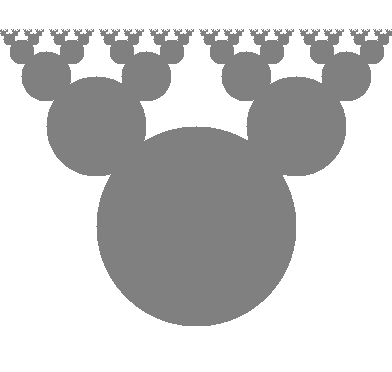
\includegraphics[height=2in]{figs/moose.png}
\caption{A recursive shape we call ``Mickey Moose''.}
\label{fig.moose}
\end{center}
\end{figure}

\end{exercise}


\begin{exercise}

In this exercise, you will draw ``Moir\'{e} patterns'' that seem to shift around as you move.
For an explanation of what is going on, see \url{https://en.wikipedia.org/wiki/Moire_pattern}.

\begin{enumerate}

\item Open {\tt Moire.java} and read the \java{paint} method.
Draw a sketch of what you expect it to do.
Now run it.
Did you get what you expected?

\item Modify the program so that the space between the circles is larger or smaller.
See what happens to the image.

\item Modify the program so that the circles are drawn in the center of the screen and concentric, as in Figure~\ref{fig.moire} (left).
The distance between the circles should be small enough that the Moir\'{e} interference is apparent.

\begin{figure}[!ht]
\begin{center}
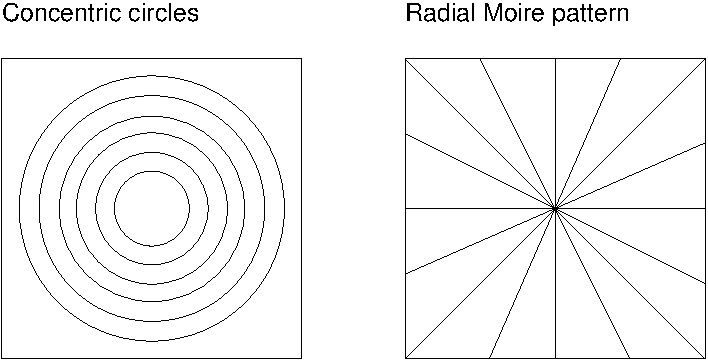
\includegraphics[height=2in]{figs/moire.pdf}
\caption{Graphical patterns that can exhibit Moir\'{e} interference.}
\label{fig.moire}
\end{center}
\end{figure}

\item Write a method named \java{radial} that draws a radial set of line segments as shown in Figure~\ref{fig.moire} (right), but they should be close enough together to create a Moir\'{e} pattern.

\item Just about any kind of graphical pattern can generate Moir\'{e}-like interference patterns.
Play around and see what you can create.

\end{enumerate}

\end{exercise}
